
In figure \ref*{fig:shift_matrix_barycentric} is plotted the $\Delta V_r^{ij}$ matrix for barycentric-corrected excalibur calibrated data for HD 34411. We are now on the order of m/s instead of km/s.

\begin{SCfigure}[1][!ht]%
    \begin{wide}  
        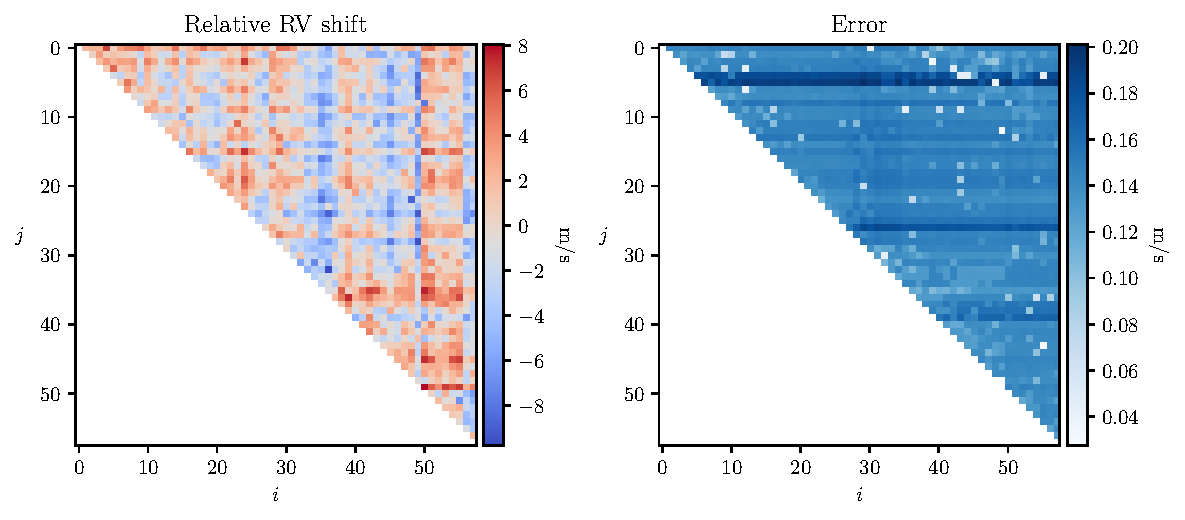
\includegraphics[width=\textwidth]{figures/shfits_matrix_bary.pdf}
        \caption{RV shifts matrix computed for HD34411 using excalibur calibrated, barycentric-corrected data (column \texttt{bary\char`_excalibur}). Each cell shows the median relative radial velocity across all features found between observations $i$ and $j$. The diagonal should be zero and has been ommited for the sake of computational speed.}
        \label{fig:shift_matrix_barycentric}
    \end{wide}
\end{SCfigure}

Performing the matrix reduction chi2 fit yields the results plotted in figure 

\begin{SCfigure}[1][!ht]%
    \begin{wide}  
        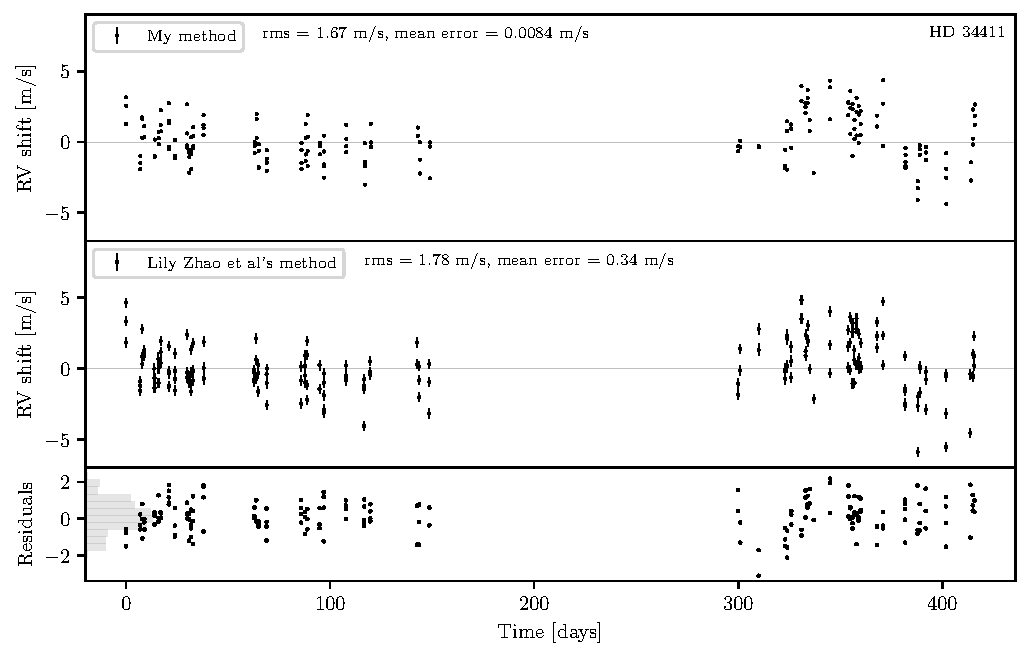
\includegraphics[width=\textwidth]{figures/HD34411_barycentric_rv_vs_lily.pdf}
        \caption{Computed relative wavelength shifts for HD34411 using excalibur calibrated, barycentric-corrected data (column \texttt{bary\char`_excalibur}). Top: my results \todo{Errors are too small}. Bottom: Lily Zhao's results using a chunk-by-chunk analysis. \todo{Cite?}}
        \label{fig:RV_results_barycentric}
    \end{wide}
\end{SCfigure}
